%!TEX root = ../report.tex

\begin{document}
    \chapter{功能效果演示}

    \section{顶点变换}
	\begin{figure}[H]
    	\centering
		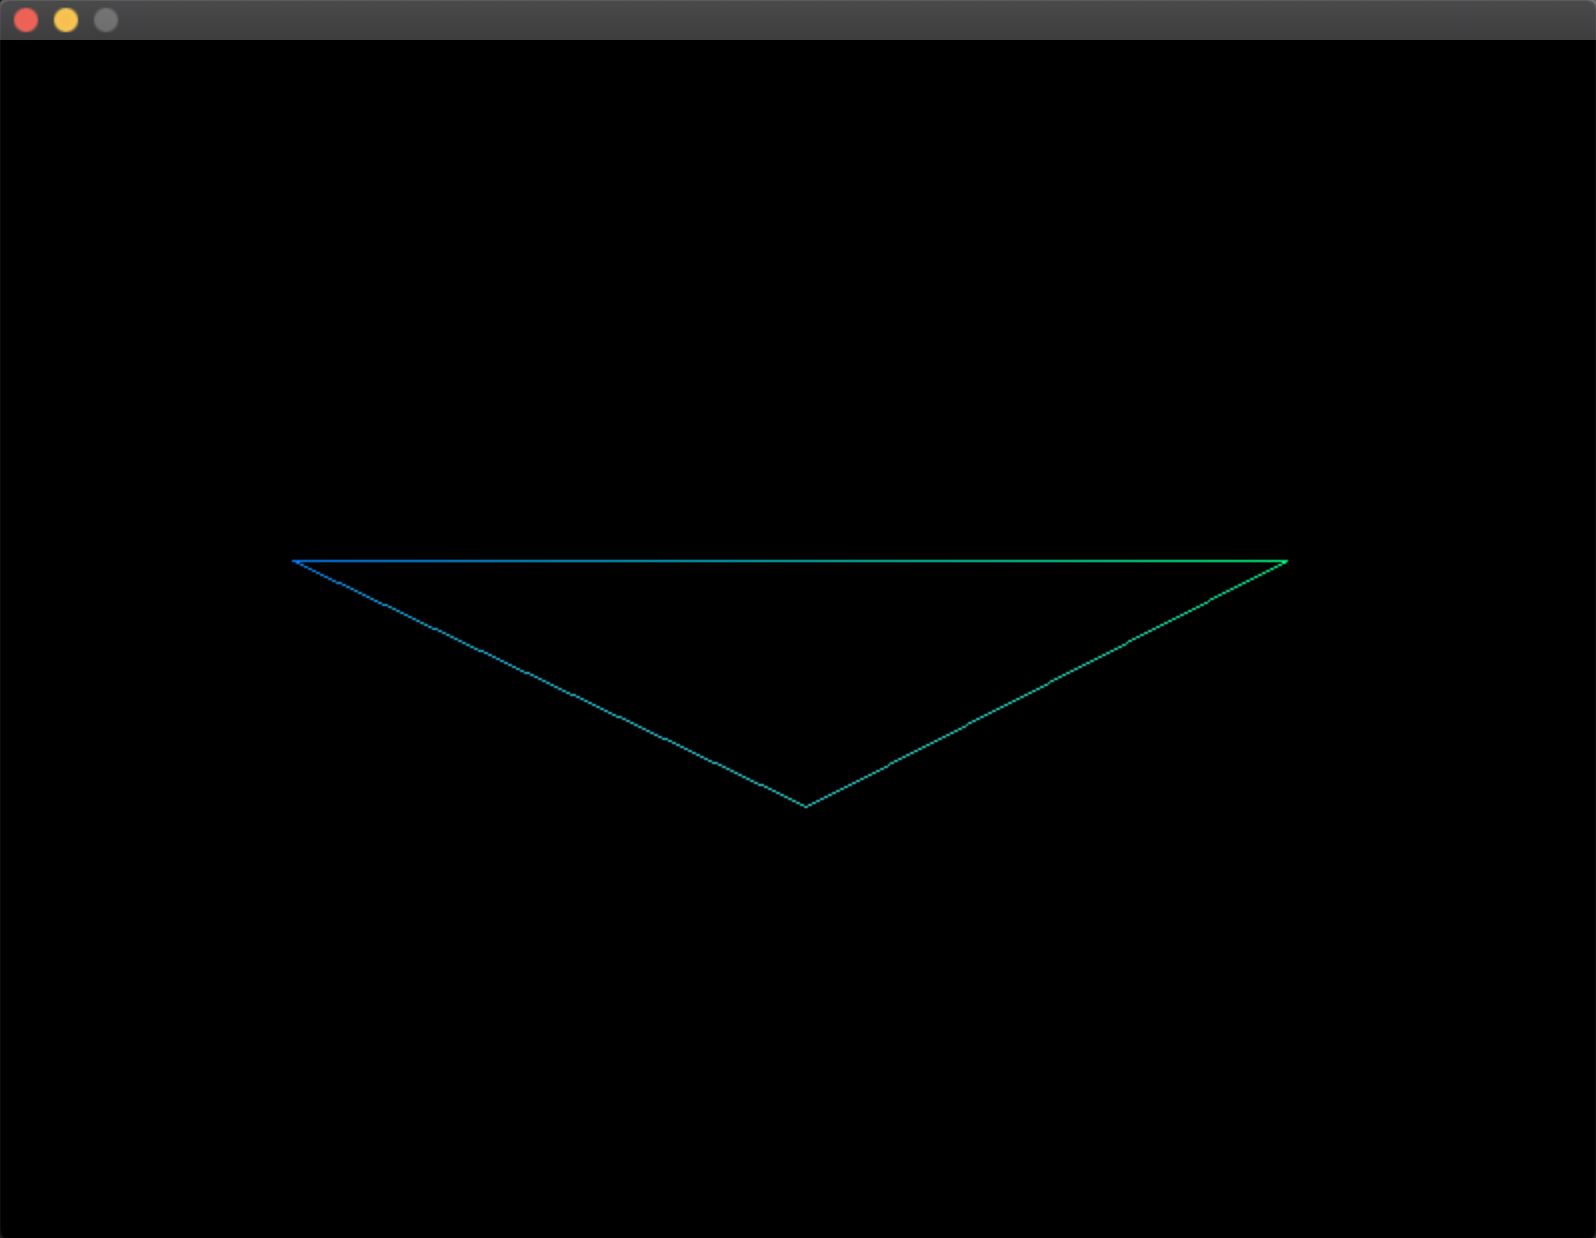
\includegraphics[width=0.8\textwidth]{images/demo1.png}
		\caption{顶点变换}
		\label{demo1}
    \end{figure}    
    
    对于每一个场景都是如此,三维的顶点变换到了二维屏幕坐标系

    \section{裁剪}
    裁剪效果如下:
    	\begin{figure}[H]
    	\centering
		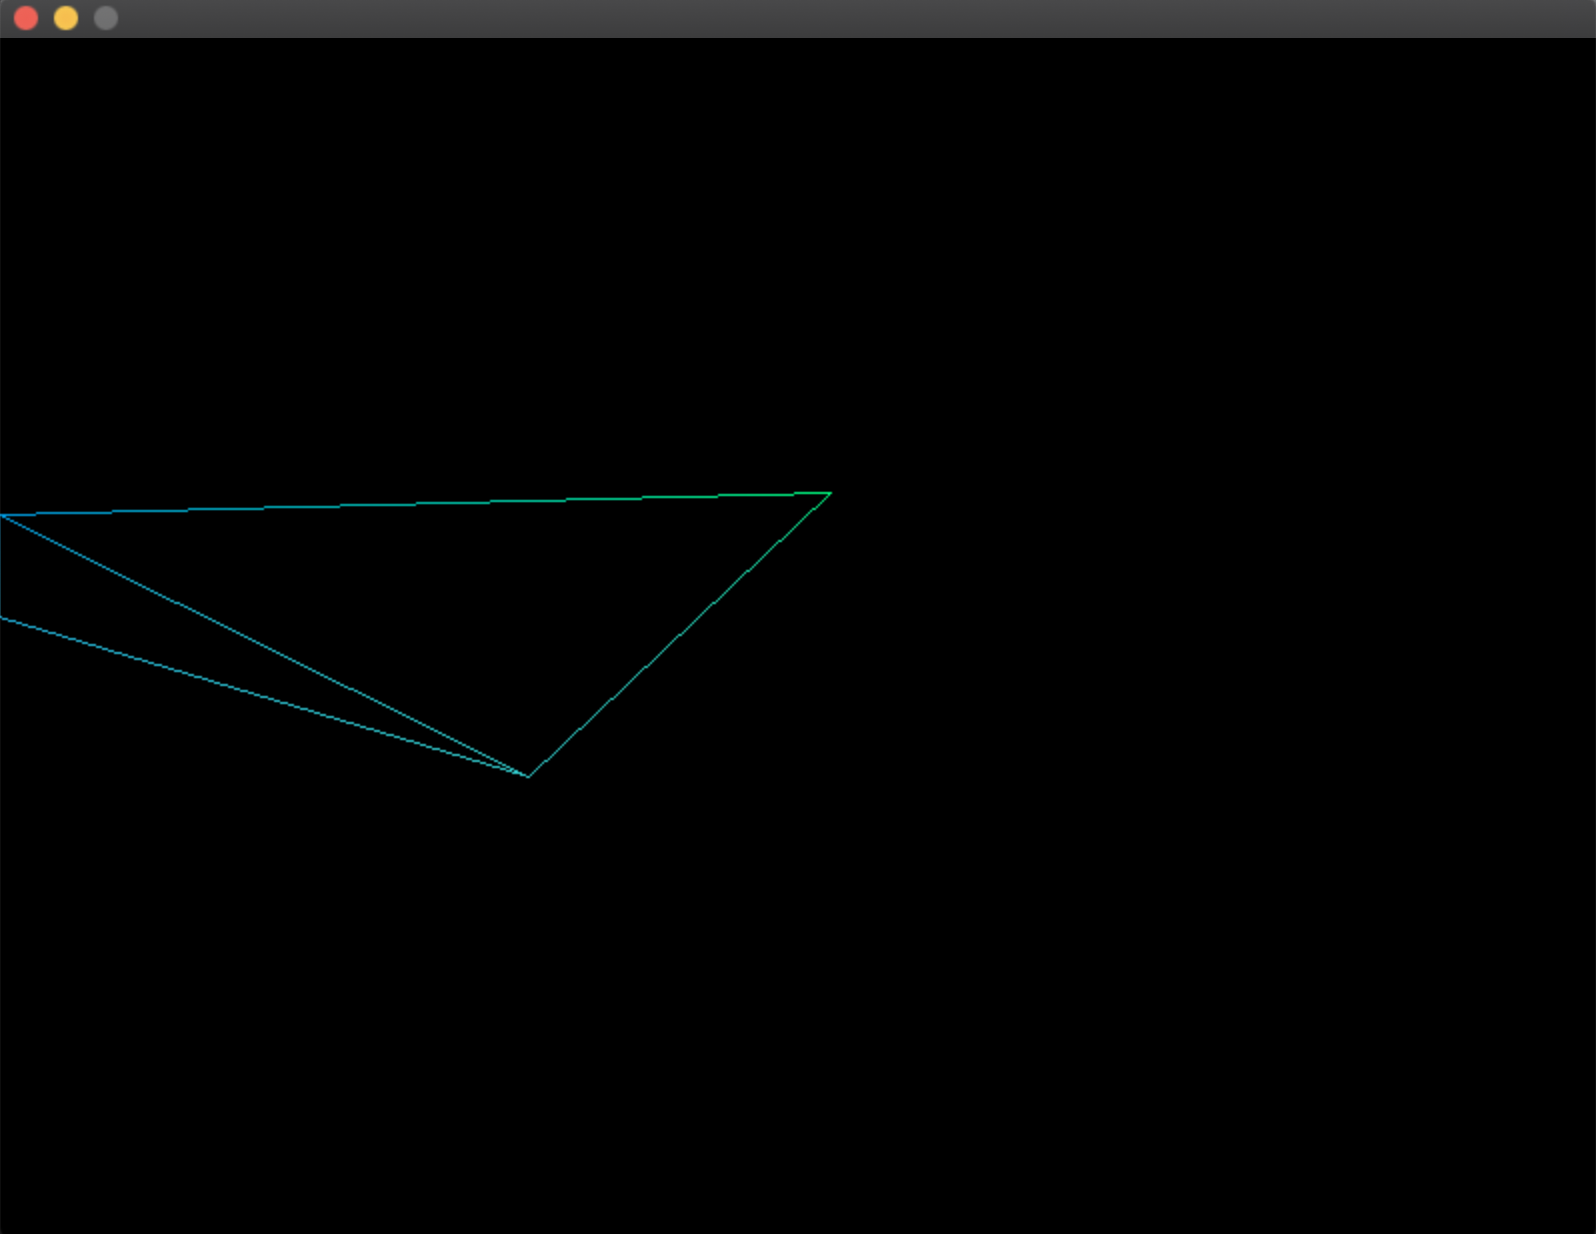
\includegraphics[width=0.8\textwidth]{images/demo2.png}
		\caption{裁剪}
		\label{demo2}
    \end{figure}  
    超出窗口边界部分将被裁剪掉。这是在CVV裁剪空间中完成的。
    	   
    \section{线框画线}
    线框画线效果如下,图中对一个正方体进行了线框描绘:
     \begin{figure}[H]
    	\centering
		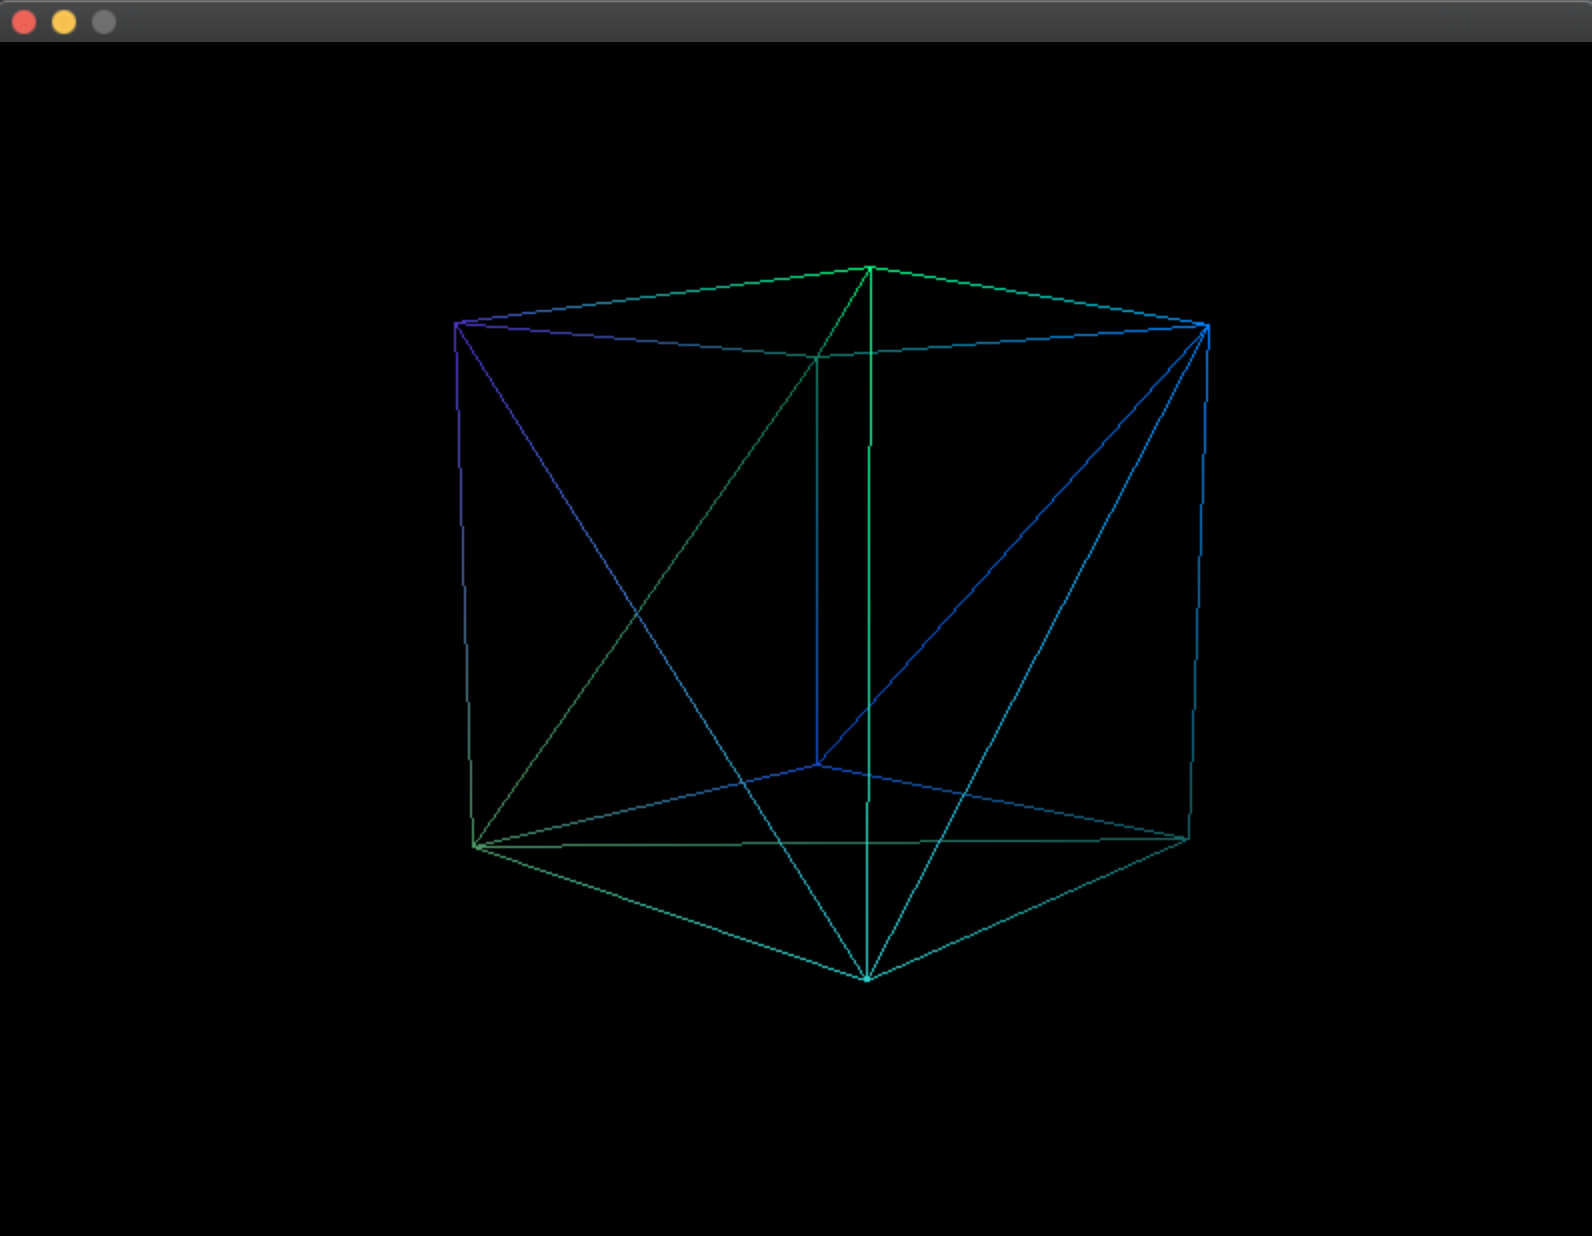
\includegraphics[width=0.8\textwidth]{images/demo3.png}
		\caption{线框画线}
		\label{demo3}
    \end{figure}  
    
    \section{键鼠交互的相机移动}
    每个场景都可以通过按键盘的上下左右/WASD或者鼠标拖动来移动物体,通过TAB键切换场景
     \begin{figure}[H]
    	\centering
		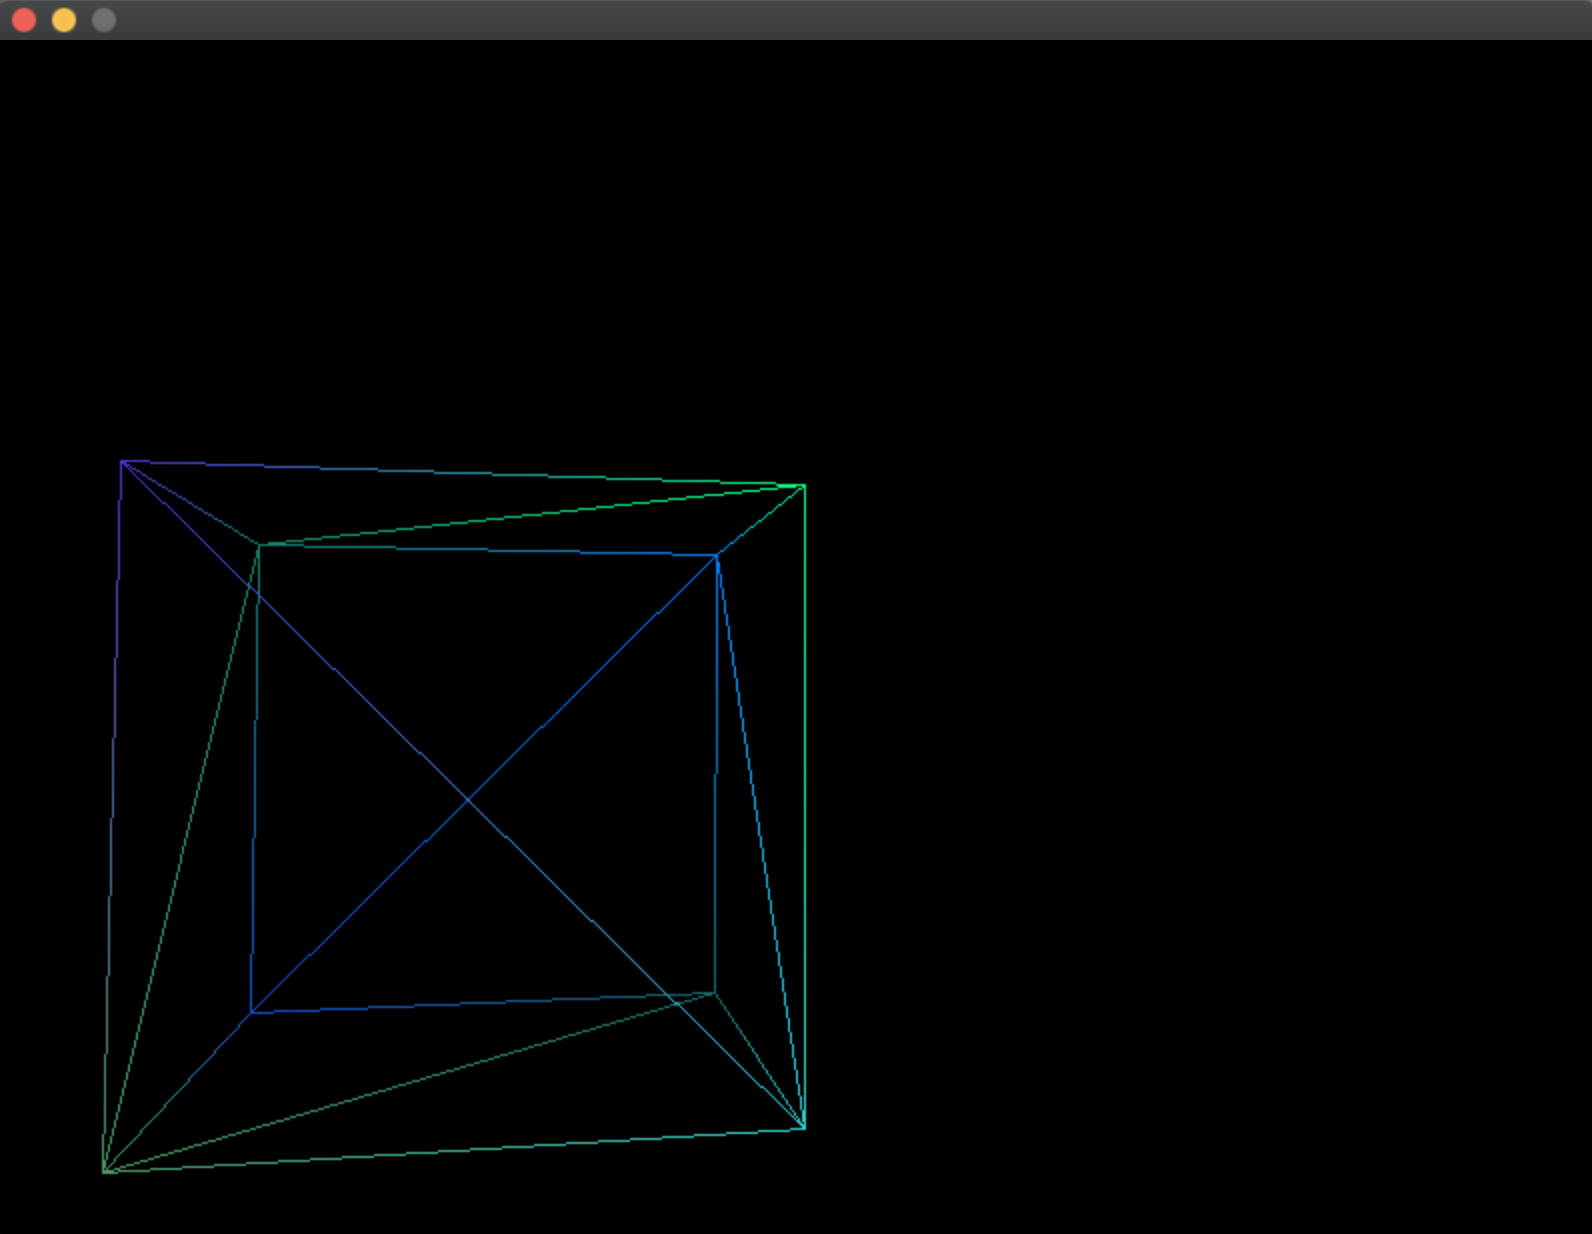
\includegraphics[width=0.8\textwidth]{images/demo4.png}
		\caption{键鼠交互的相机移动}
		\label{demo4}
    \end{figure}  
 
    \section{扫描线填充}
    除了线框画线,我们还可以对图形进行扫描线填充,通过给予顶点初始颜色值,我们可以用扫描线算法对区域中每一个像素点进行着色,其中颜色值由片元着色器根据顶点颜色插值得到。
        \begin{figure}[H]
    	\centering
		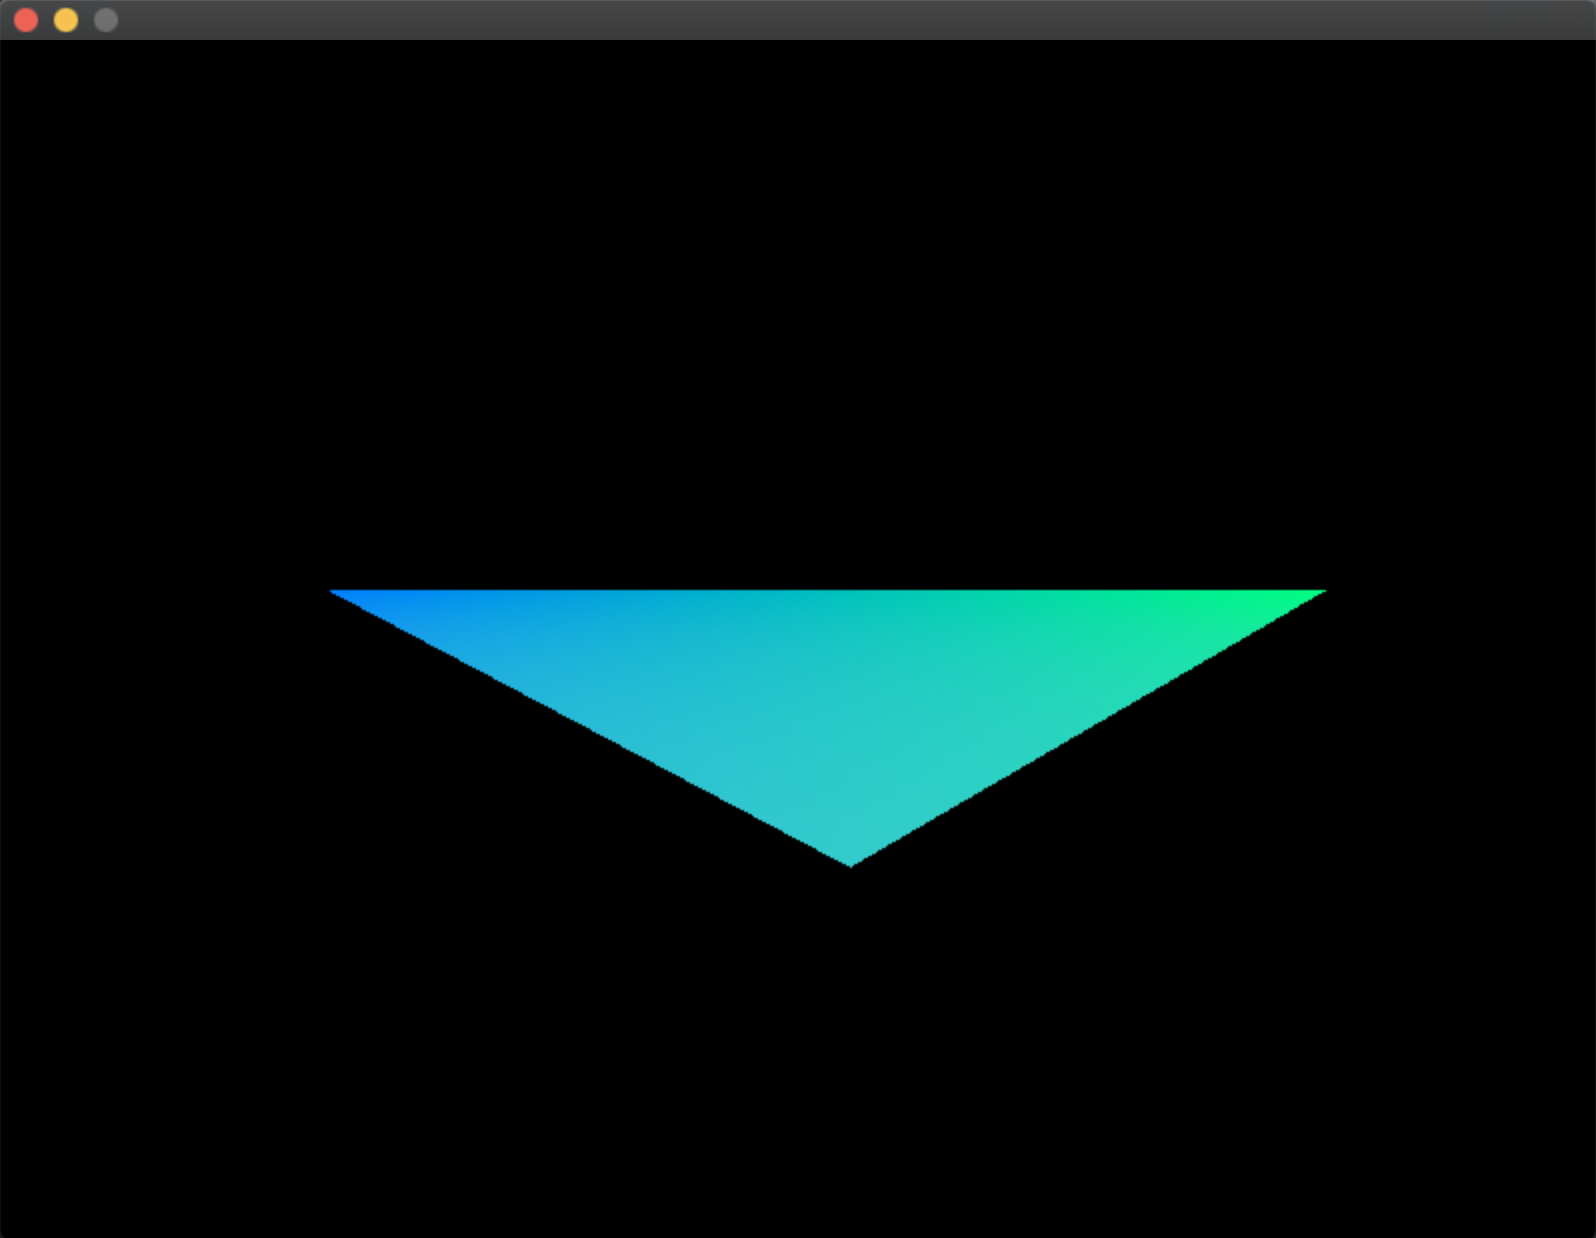
\includegraphics[width=0.6\textwidth]{images/demo5.png}
		\caption{扫描线填充1}
		\label{demo5}
    \end{figure}  
    
        \begin{figure}[H]
    	\centering
		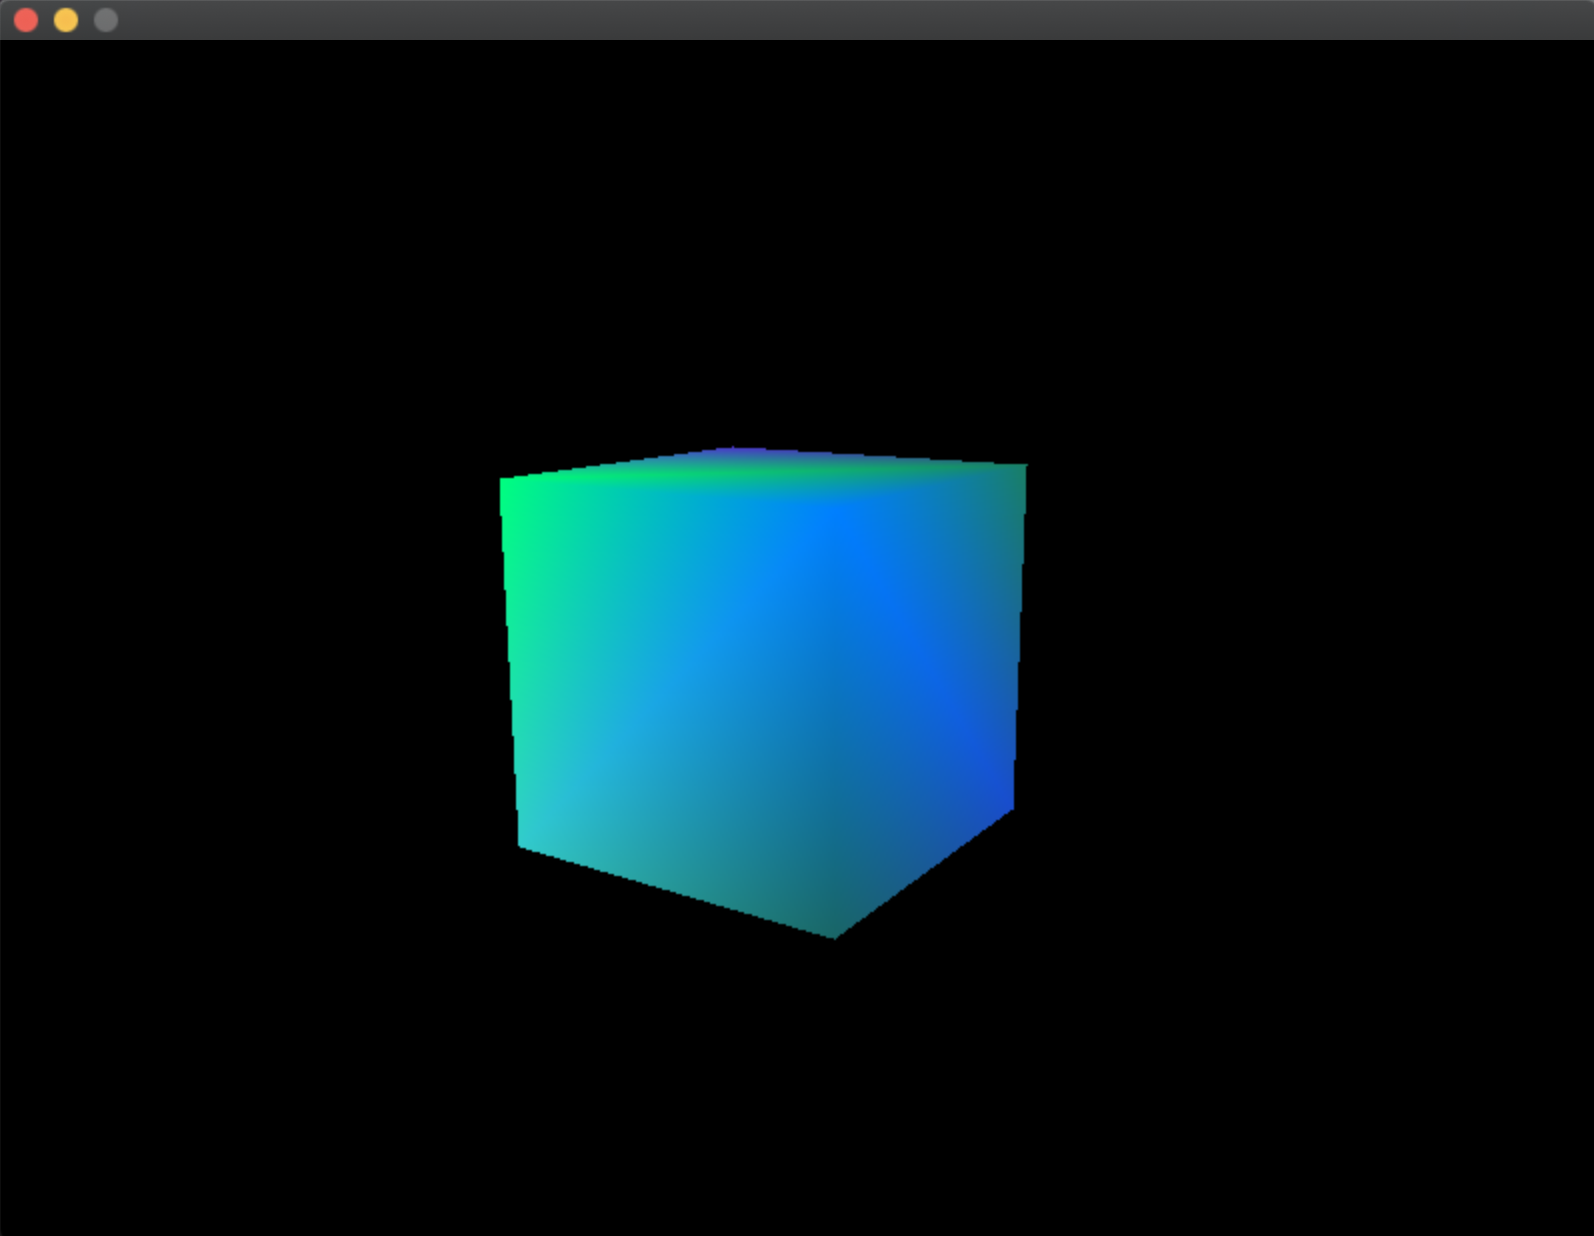
\includegraphics[width=0.6\textwidth]{images/demo11.png}
		\caption{扫描线填充2}
		\label{demo11}
    \end{figure} 
    
    \section{纹理贴图}
    按照前面所述的纹理贴图流程进行贴图的结果如下:
        \begin{figure}[H]
    	\centering
		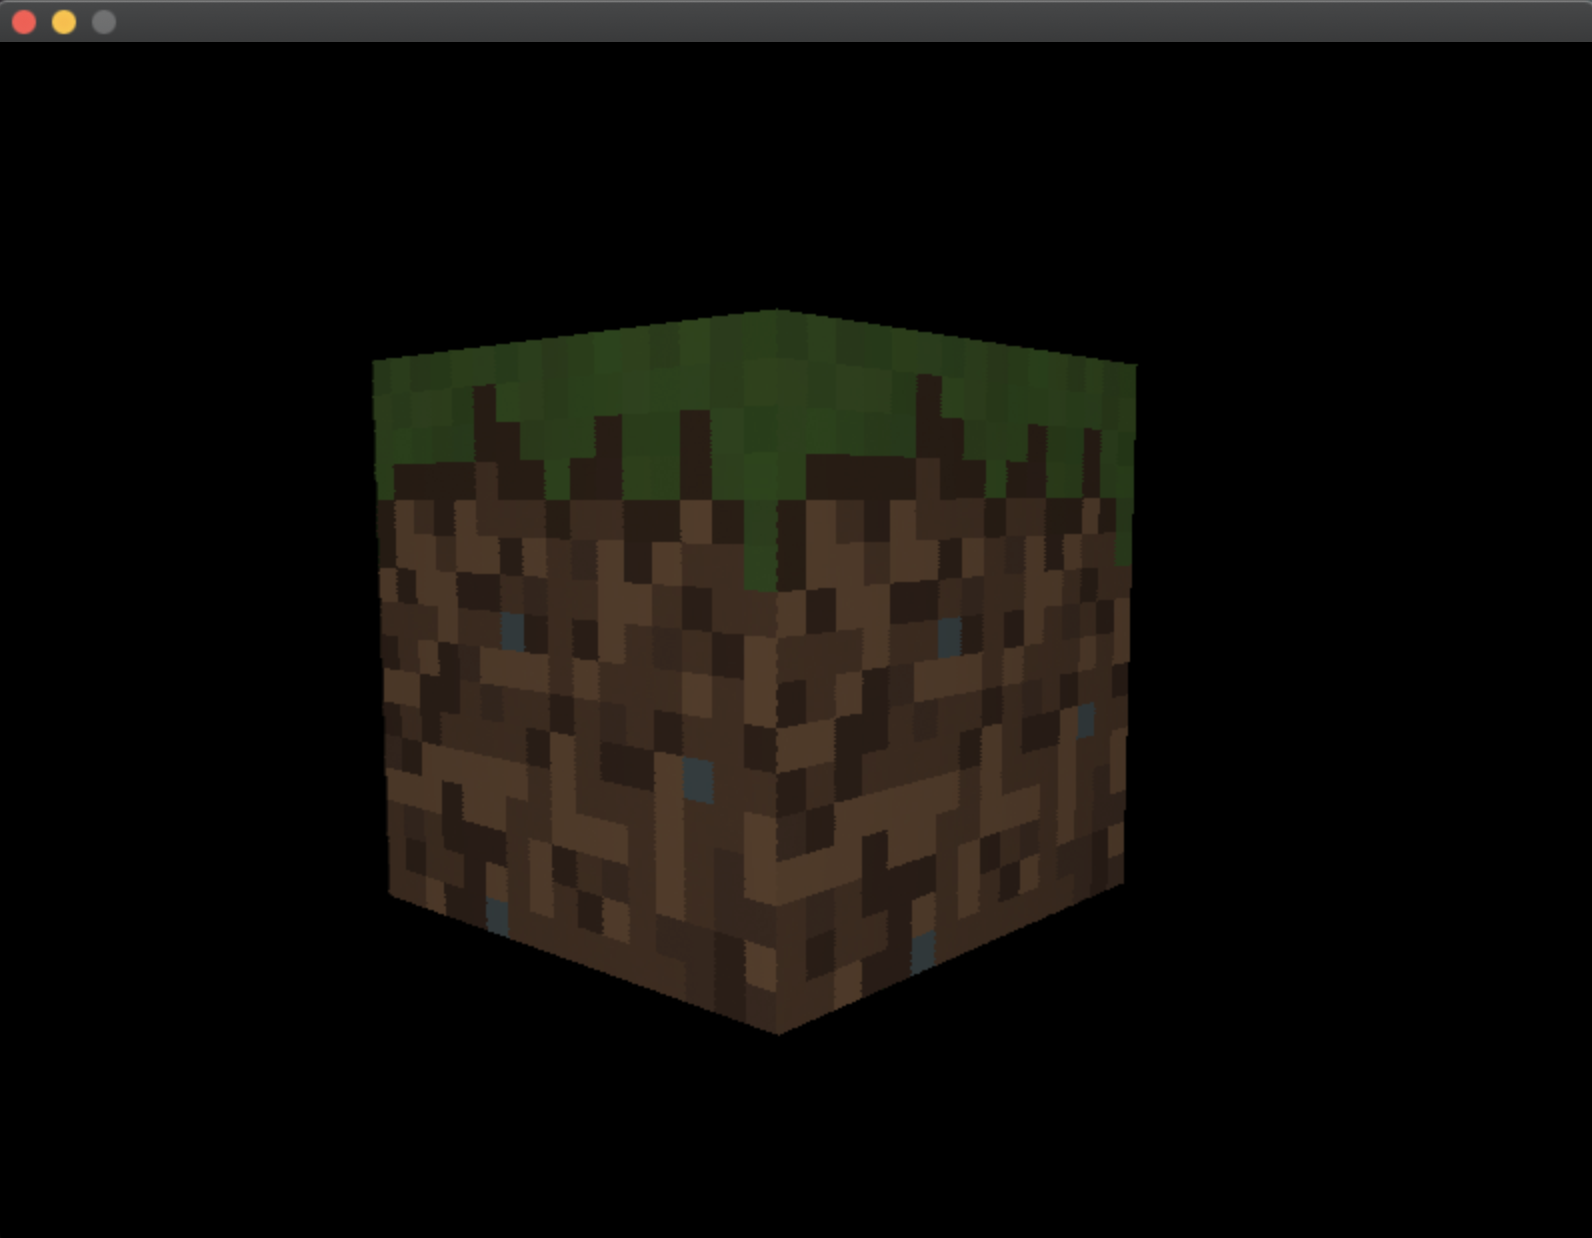
\includegraphics[width=0.8\textwidth]{images/demo6.png}
		\caption{纹理贴图}
		\label{demo6}
    \end{figure} 
    
    \section{光照}
    给模型添加光照后,可以得到如下效果:
        \begin{figure}[H]
    	\centering
		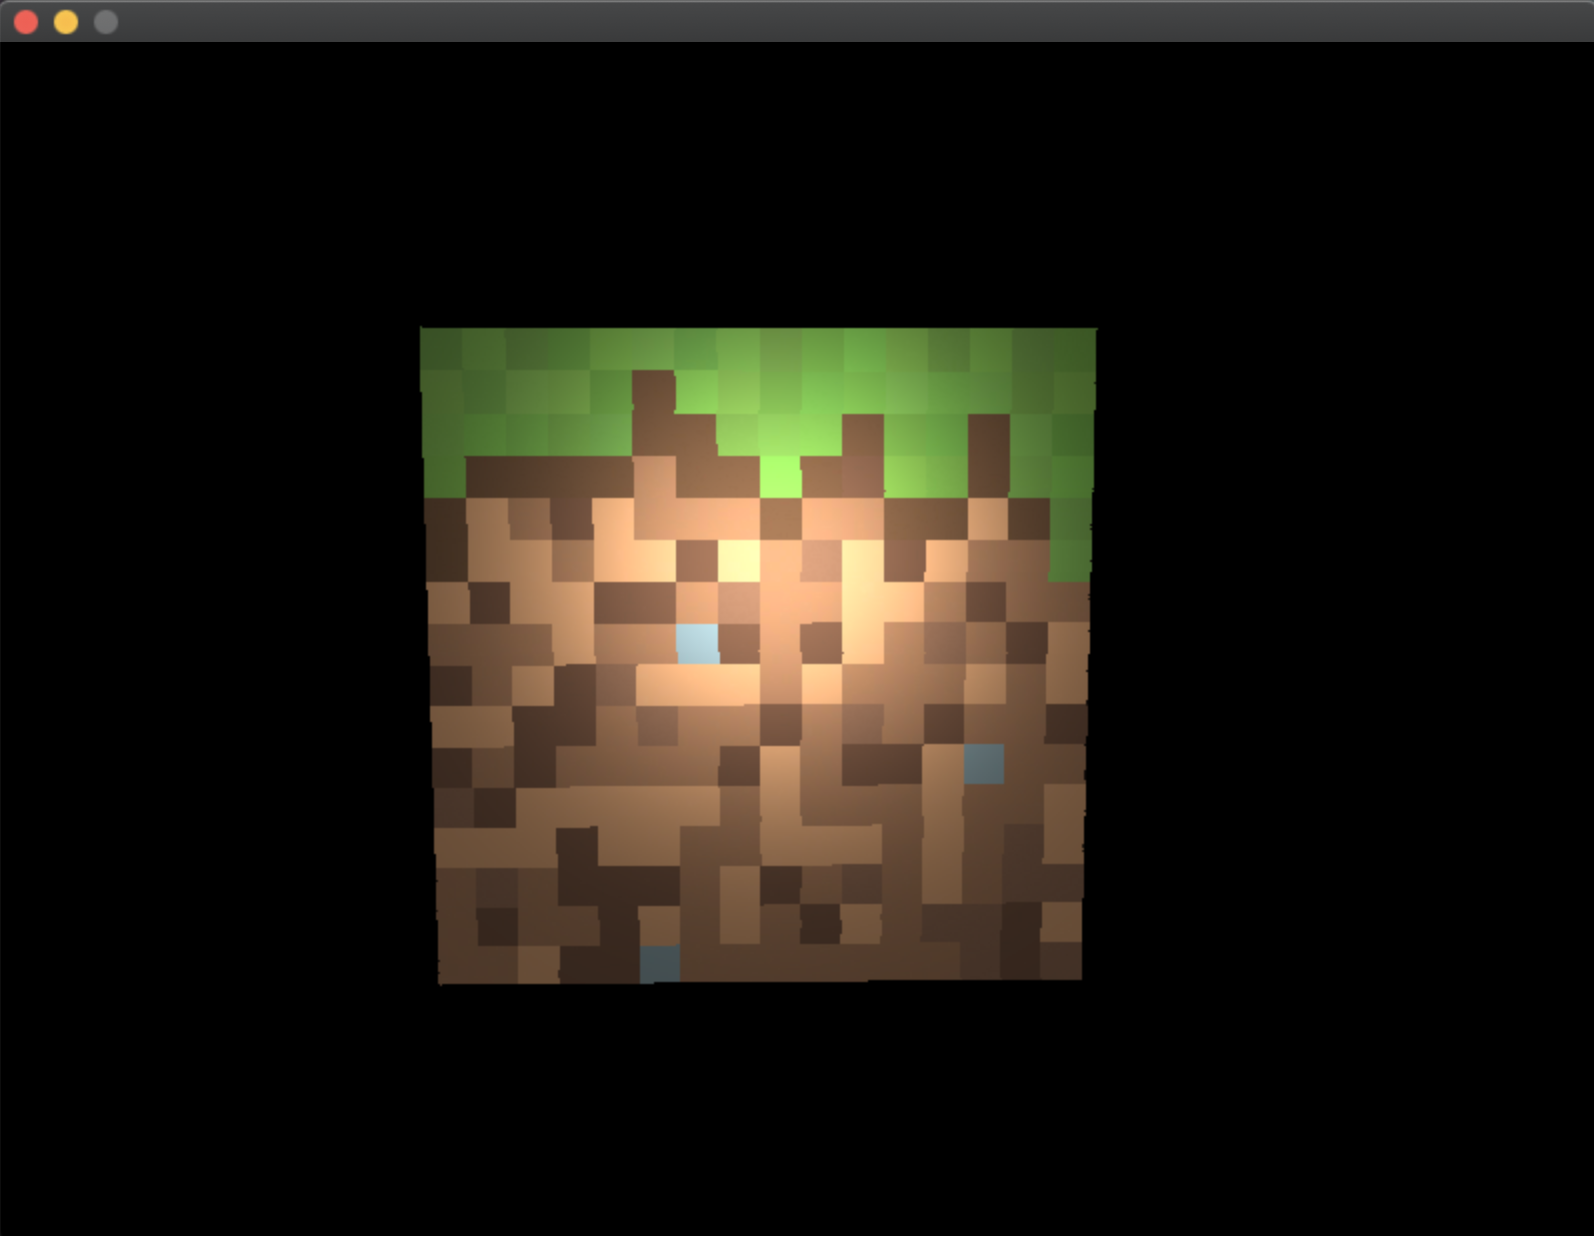
\includegraphics[width=0.8\textwidth]{images/demo7.png}
		\caption{光照}
		\label{demo7}
    \end{figure} 
    
    \section{三维模型}
    我们自己制作了一个同济Logo的三维模型,然后导入了光栅渲染器中,并也加上了光照。
            \begin{figure}[H]
    	\centering
		
\includegraphics[width=0.8\textwidth]{images/demo8.png}
		\caption{三维模型}
		\label{demo8}
    \end{figure} 
    
    \section{天空盒子}
    最后就是天空盒子,可以让人有身临其境之感:
            \begin{figure}[H]
    	\centering
		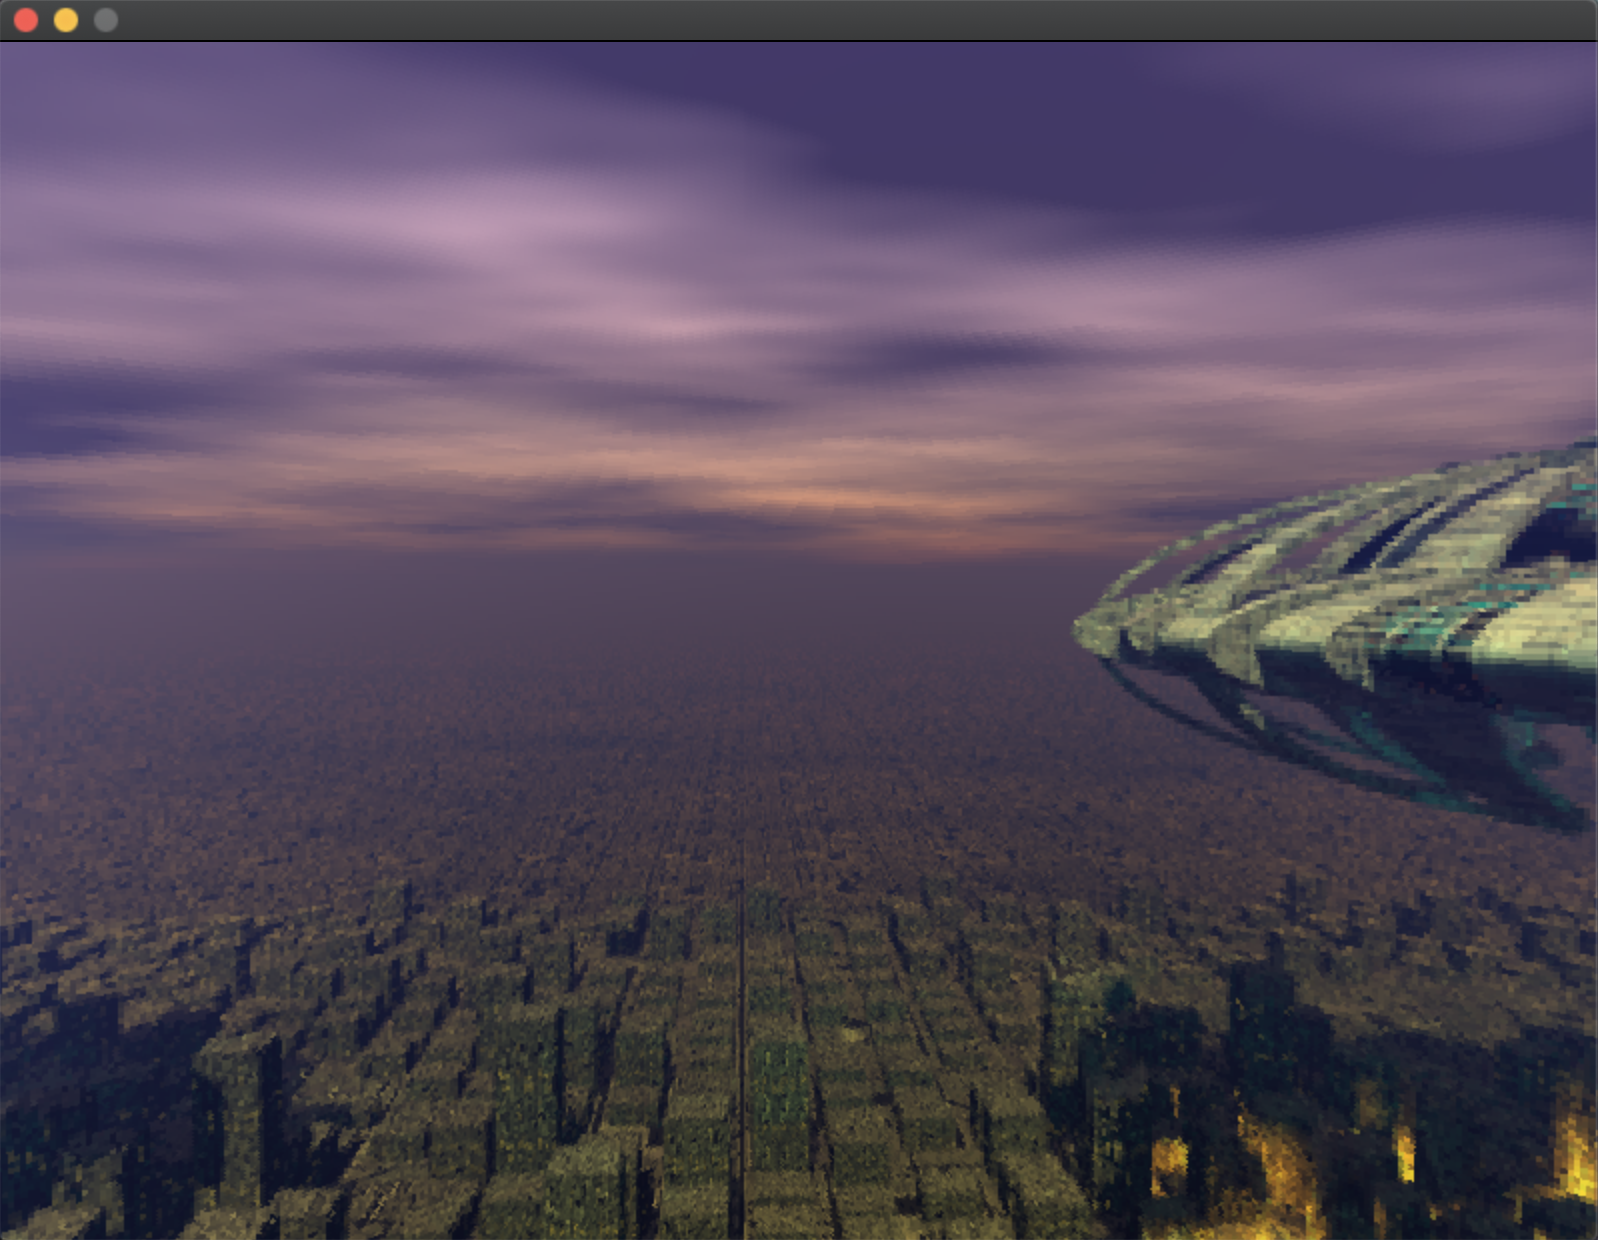
\includegraphics[width=0.7\textwidth]{images/demo9.png}
		\caption{天空盒子1}
		\label{demo9}
    \end{figure} 
    
                \begin{figure}[H]
    	\centering
		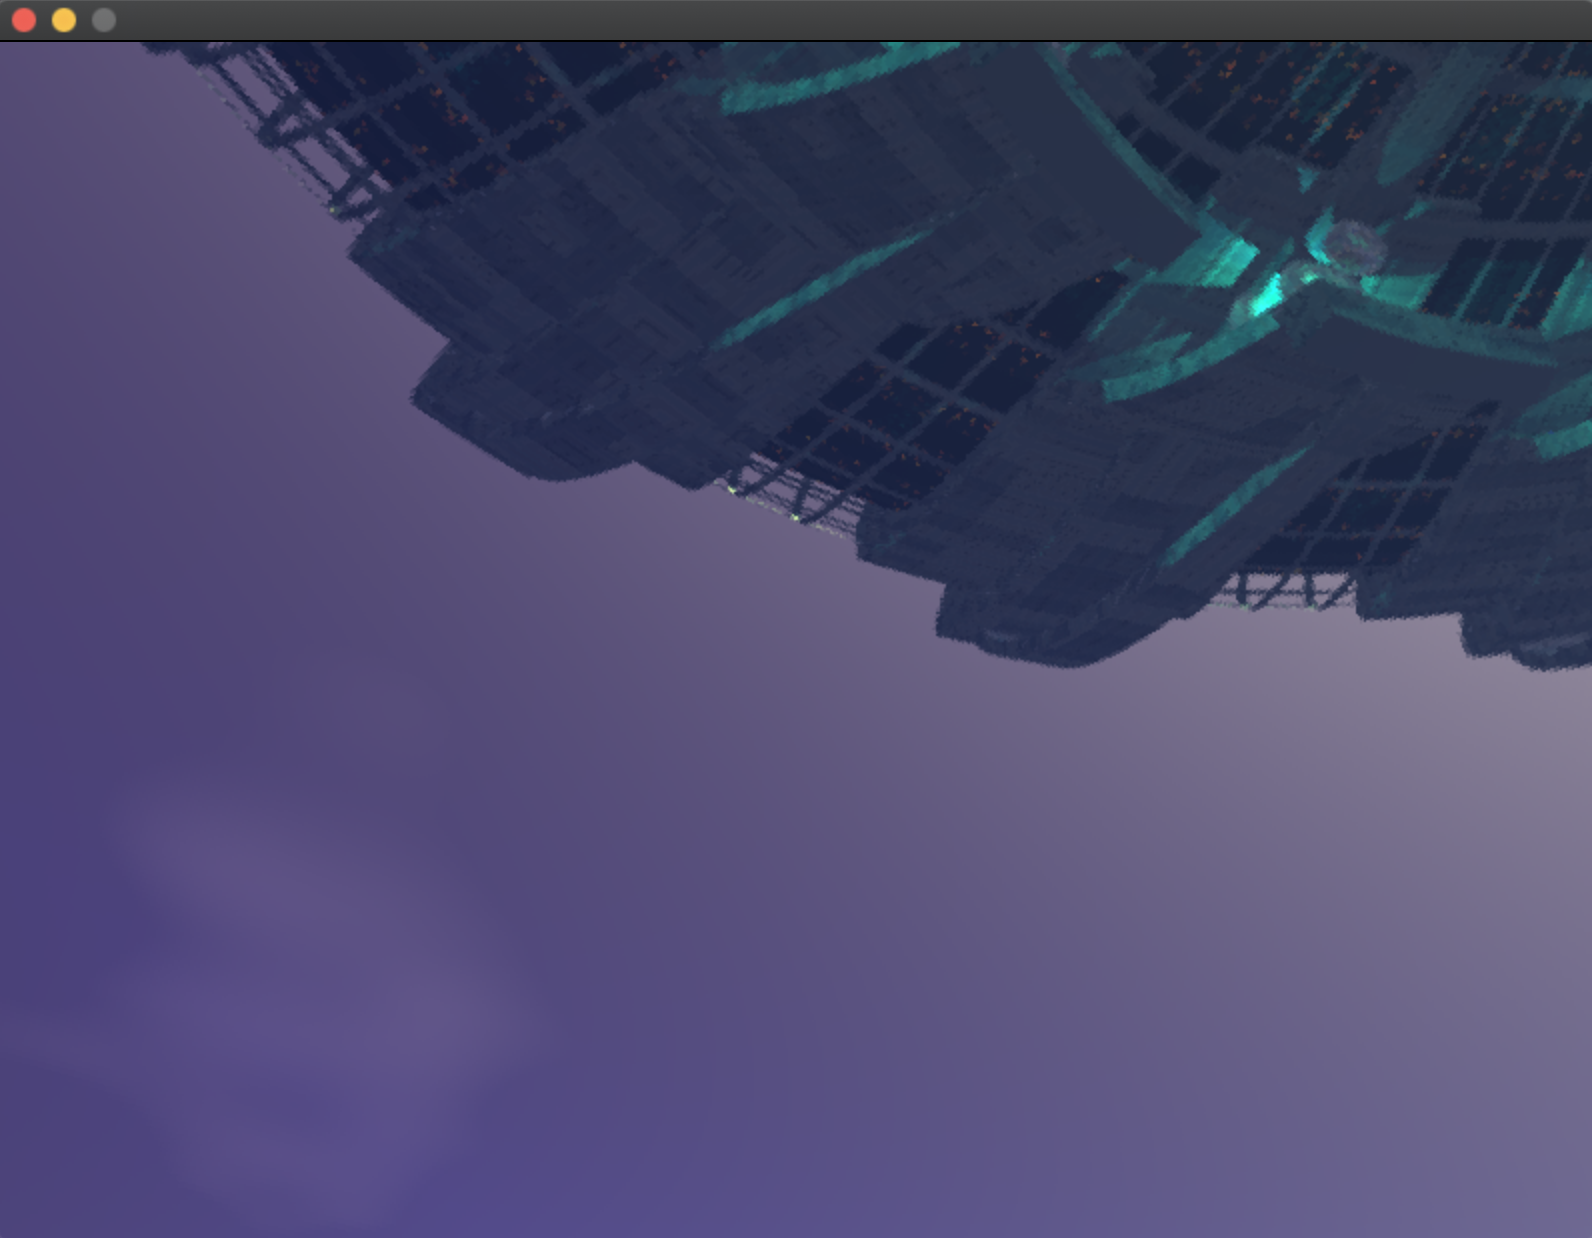
\includegraphics[width=0.7\textwidth]{images/demo10.png}
		\caption{天空盒子2}
		\label{demo10}
    \end{figure} 
\end{document}
